%set ukuran paper jadi a4 sama 12 pixel font
\documentclass[f4paper,12pt, left=3cm,right=2cm,bottom=2cm, bahasa]{article}
\usepackage{graphicx} % Required for inserting images
\usepackage[utf8]{inputenc}

\usepackage[autostyle]{csquotes}

%hyprlink desuwa
\usepackage{hyperref}
\hypersetup{
    colorlinks,
    citecolor=black,
    filecolor=black,
    linkcolor=black,
    urlcolor=black
}
%ganti jadi roman
\usepackage{times}

%set margin
 \usepackage{geometry}
 \geometry{margin=2cm}

%set bahasa indonesia
%\captionsbahasa
% \usepackage[american]{babel}


%biber dsw
% \usepackage[backend=biber,style=apa, sorting=none]{biblatex}
% \addbibresource{./ref.bib}


%set spacing 1.5
 \usepackage{setspace}
 \onehalfspacing{}
\usepackage{tocloft}

%bikin tabel berwarna
\usepackage[table,xcdraw]{xcolor}
\renewcommand{\cftpartleader}{\cftdotfill{\cftdotsep}}

%bikin judul utama centering
\usepackage{titlesec}
\titleformat{\section}[hang]{\normalfont\Large\bfseries}{\thesection}{1em}{\centering}
%idk harus pake date biar gak nongol di title
\date{}

%judul dokumen
\title{Proses Pembuatan Yogurt\\ Praktikum Bioteknologi Konvensional}

\begin{document}

%bikin judul jalan
\maketitle
%bikin page ini ga pake nomor
\thispagestyle{empty}
% logo
\begin{figure}[ht]
    \centering
    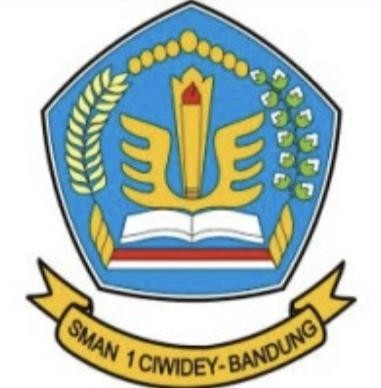
\includegraphics[width=0.3\linewidth]{images/sman1.png}
\end{figure}
%vertical space 2 cm

%nama penulis
\begin{center}
    Kelompok 2 : \\
    \begin{tabular}{ll}
         1.& Hasby Nauril Atoriq  \\
         2.& Abdan Fakih Makhlufi \\
         3.& Rezza Rahmadani \\
         4.& Riana Nur Rahmadina \\
         5.& Jihan Fathimatul Zahra\\
    \end{tabular}\\
    \vspace{0.5cm}
    Kelas X-1\\
    \vspace{1cm}
    \textbf{PEMERINTAH DAERAH PROVINSI JAWA BARAT}\\
    \textbf{DINAS PENDIDIKAN}\\
    \textbf{SMA NEGERI 1}
    \textbf{CIWIDEY}\\
    \textbf{2024}
\end{center}
\pagebreak
\onehalfspacing{}
\section*{KATA PENGANTAR}
%ganti nomor jadi romaj
\pagenumbering{Roman}
\setcounter{section}{1}
\addcontentsline{toc}{section}{\protect\numberline{}KATA PENGANTAR}


Assalamualaikum Wr. Wb. Puji syukur kehadirat Allah SWT atas segala rahmat dan hidayah-Nya sehingga penulis dapat menyelesaikan tugas bimbingan konseling ini dengan judul “Pentingnya Kedisiplinan di Sekolah”. Tugas ini disusun sebagai salah satu persyaratan untuk memenuhi tugas mata pelajaran Bahasa Indonesia. 

Disiplin merupakan salah satu nilai penting yang harus dimiliki oleh setiap individu, terutama siswa. Dalam konteks pendidikan, kedisiplinan memiliki peran yang sangat krusial dalam membentuk karakter dan prestasi siswa. Melalui tugas ini, penulis berusaha untuk mengkaji lebih dalam mengenai pentingnya kedisiplinan di sekolah serta dampaknya terhadap kehidupan siswa. Penulis menyadari bahwa tugas ini masih jauh dari sempurna. Oleh karena itu, penulis sangat mengharapkan kritik dan saran yang membangun dari berbagai pihak. Semoga tugas ini dapat bermanfaat bagi semua pihak. Wassalamualaikum Wr. Wb.\\
    
\rightline{Pasirjambu, November 2024}
\vspace{3cm}
\rightline{Kelompok 2}
\pagebreak

    \section*{DAFTAR ISI}
    \addcontentsline{toc}{section}{\protect\numberline{}DAFTAR ISI}
% \end{center}
\renewcommand{\cftdot}{.}
\tableofcontents



%\vspace{3cm}
%\section*{DAFTAR PUSTAKA}
%\addcontentsline{toc}{section}{\protect\numberline{}DAFTAR PUSTAKA}
%\medskip
%\printbibliography

\pagebreak
\pagenumbering{arabic}
\setcounter{page}{1}
\setcounter{section}{1}


\section*{BAB I \\PENDAHULUAN}
\addcontentsline{toc}{section}{\protect\numberline{}BAB I PENDAHULUAN}
Sekolah merupakan sebuah wadah bagi pemerintah untuk merealisasikan pendidikan nasional yang diperuntukan oleh masyarakat.
hal ini menjadikan sekolah diharuskan membuat tata tertib untuk mengatur jalannya pendidikan agar berjalan sesuai dengan tujuan yang hendak dicapai. hal ini sesuai dengan Undang-undang tentang Sistem Pendidikan Nasional Bab V. Pasal 12, Ayat(2a) yang menjelaskan bahwa, setiap peserta didik berkewajiban menjaga norma-norma pendidikan untuk menjamin keberlangsungan proses dan keberhasilan pendidikan.

Alasan sekolah membuat tata tertib karena sekolah mempunyai tugas 
menjamin keberlangsungan proses dan keberhasilan pendidikan setiap siswa. 
Tentu saja tata tertib tidak akan berguna jika siswa-siswi tidak disiplin. Hal ini 
menyebabkan disiplin menjadi kunci siswa-siswi dapat mematuhi tata tertib. 

Tata tertib sekolah seharusnya mengajarkan apa yang boleh dilakukan dan tidak \cite{Widi_et_al_2018}
boleh dilakukan di sekolah mapun diluar sekolah ketika guru tidak dapat 
mengawasi. Tata tertib yang berlaku di sekolah harus diberikan secara jelas dan 
tegas kepada siswa, agar mereka dapat mematuhi sesuai dengan tujuan atau 
harapan sekolah

Tata tertib yang dibuat sekolah adalah upaya sekolah untuk membentuk 
karakter disiplin pada siswa karena sekolah merupakan tahap selanjutnya 
setelah pembentukan karakter oleh orang tua. Disiplin juga mempunyai dampak 
yang baik bagi anak dan kedepannya.\cite{tu2004peran} mengatakan perencanaan dan  implementasi
disiplin sekolah akan berdampak memelihara siswa selalu berada dalam tugasnya; membantu siswa bersikap dan bertingkah laku penuh tanggung jawab serta sesuai dengan disiplin yang berlaku di sekolah, membimbing dan mengarahkan serta mendorong para siswa bertingkah laku yang baik sehingga ada pertumbuhan pribadi yang baik pula, mencegah dan menekan serta meluruskan tingkah laku yang salah, mengusahakan hubungan yang baik di antara para siswa. 
Disiplin merupakan salah satu aspek yang sangat penting bagi keberhasilan prestasi 
akademik siswa . Disiplin sekolah berperan penting dalam pencapaian harapan dan 

Pihak sekolah jika menerapkan kedisplinan dengan baik maka sebenarynya akan mempunyai banyak manfaat. Salah satu manfaat menurut  \cite{Hurlock_1991} disiplin adalah cara untuk mendidik individu untuk mengembangkan kontrol diri dan arah diri serta mampu menyesuaikan diri dengan harapan yang diterima di lingkungan sosialnya sehingga individu dapat bertindak dan mengambil keputusan dengan bijaksana. Hal ini berarti apabila pendidik dapat mengontrol siswa dengan baik maka kedisiplinan merupan merupakan proses untuk membantu anak mengubah tingkah lakunya ke arah yang lebih baik. \cite{njoroge_2014}

Kedisiplinan sebenarnya mempunyai tujuan yang mulia dan kedisiplinan juga mendukung fungsi dari pendidikan nasional, 
tetapi setiap individu mempunyai tingkat kedisiplinan yang berbeda-beda, perbedaan tersebut karena di dalam kedisiplinan terdapat faktor-faktor yang mempengaruhinya, faktor-faktor kedisiplinan menurut \cite{tu2004peran} :
\begin{enumerate}
  \item Kesadaran diri sebagai pemahaman diri bahwa disiplin dianggap penting bagi kebaikan dan keberhasilan diri
  \item Pengikutan dan ketaatan sebagai langkah penerapan dan praktik atas peraturan pertauran yang mengatur perilaku individu
  \item alat pendidikan untuk mempengaruhi, mengubah, membina dan membentuk perilaku yang sesuai dengan nilai-nilai yang ditentukan atau diajarkan
  \item hukuman sebagai upaya penyadaran, mengkoreksi dan meluruskan yang salah sehingga orang kembali pada perilaku yang sesuai dengan harapan 
\end{enumerate}

pada faktor disiplin poin ketiga, kedisiplinan juga ditentukan oleh alat pendidikan yang digunakan untuk mempengaruhi, merubah, membentuk perilaku. Fungsi dari disiplin juga untuk mempengaruhi, merubah, membentuk perilaku. Fungsi dari disiplin juga membangun dan melatih kepribadian. Hal tersebut senada dengan hasil penelitian oleh \cite{Sumantri_2010}  yang mengungkapkan tingkat kedisiplinan siswa dalam belajar merupakan salah satu faktor yang ikut mempengaruhi terhadap prestasi belajar siswa, semakin tinggi tingkat disiplin belajar semakin tinggi pula prestasi belajar yang dicapainya. 

Poin pertama dari faktor kedisiplinan di atas adalah kesadaran disi, akan tetapi tidak dapat dipungkiri bahwa sampai saat ini banyak siswa-siswi belum sadar akan pentingnya kedsiplinan. Hal ini menyebabakan masih banyak perilaku siswa-siswi yang tidak disiplin dan melanggar tata tertib sekolah \cite{Samani_Hariyanto} mengungkapkan bahwa pelanggaran terhadap berbagai aturan dan tata tertib sekolah masih sering seperti tawuran antar pelajar, pemerasan / kekerasan \textit{(bullying)}, penggunaan narkoba, krisis kejujuran, mencontek, seks bebas, bolos dan penyimpangan lainnya. 

meskipun dengan banyaknya keuntungan dari jalannya sistem kedisiplinan di sekolah ini, seringkali siswa tidak pernah dilibatkan dalam perumusan tata tertib ini, mereka yang menjadi objek tata tertib ini tidak diikutsertakan dalam proses perumusan ini dapat menyebabkan ketidak selarasan antara tata tertib dengan kebutuhan siswa. Siswa hanya berperan sebagai pelaksana tanpa mengetahui dasar tata tertib sekolah. oleh karena itu para siswa tidak memiliki pemahaman sama sekali mengenai tata tertib dan menganggap remeh terhadap ketidakdisiplinan menjadi faktor yang melatar belakangi pelanggaran tata tertib \cite{anzalena2019faktor} . selain itu sekolah masih diwarnai berbagai kasus pelanggaran berat seperti tindak kekerasan yang diklakukan antarsiswa, guru terhadap siswa atau bahkan siswa terhadap guru. Berdasarkan data dari Kementrian Pemberdayaan Perempuan Dan Perlindungan Anak menunjukan bahwa 67\% siswa menyatakan pernah melakukan kekerasan, 27\% guru laki-laki dan 17\% guru perempuan menjadi pelaku kekerasan fisik di sekolah \cite{widodo2017sekolah}. data tersebut menunjukan bahwa pelanggaran tata tertib tidak hanya oleh siswa saja namun dapat terjadi dengan guru. 



\pagebreak

\section*{BAB II \\ DAMPAK POSITIF KEDISIPLINAN}
\setcounter{section}{2}
\addcontentsline{toc}{section}{\protect\numberline{}BAB II Dampak Positif Kedisiplinan}
Tidak dapat dipungkiri bahwa kedisiplinan yang diterapkan dengan adanya tata tertib di sekolah akan menghasilkan hasil yang positif bagi para siswa-siswi yang dapat berdampak baik bagi aktivitas akademik mereka di sekolah yang kemudian dapat membentuk mereka menjadi individu yang baik dan dapat berguna bagi masyarakat dan dapat memberikan hasil yang baik kepada masyarakat dan sekitarnya, dengan begitu maka ada beberapa dampak baik dari implementasi kedisiplinan di area sekolah yakni:
\subsection{Peningkatan Prestasi Akademik}
Berdasarkan penelitian yang dilakukan oleh  \cite{zimmerman2014comparing} menyatakan bahwa siswa yang disiplin memiliki prestasi akademik yang baik sehingga kedisiplinan siswa itu selaras dengan prestasi akademik anak tersebut. oleh sebab itu maka jika dilaksanakan dengan benar sistem kedisiplinan ini dapat mengarahkan para siswanya menjadi siswa yang lebih baik dan dapat menfokusnya para siswa untuk meraih mimpi mereka untuk masa depan yang baik dan dapat menjadi sebuah acuan dalam nanti di kehidupan bermasyarakat sehingga mereka tidak terjerumus dengan kegiatan yang berbahaya seperti mengikuti perkumpulan gang motor, mengkonsumsi narkoba dan pergaulan bebas \cite{ariananda2014pengaruh}


\subsection{Perkembangan Karakter Yang Baik}
jamal Ma'mur Asmani \cite{samrin2016pendidikan} menjelaskan bahwa karakter adalah kepribadian ditinjau dari titik tolak etis atau moral. karakter memeiliki kesamaan arti dengan moral. Moral merupakan Kondisi pikiran, perasaan ucapan dan perilaku manusia yang terkait dengan nilai-nilai baik dan buruk. Berdasarkan definisi tersebut maka dapat disimpulkan bahwa pendidikan karakter merupakan usaha yang dilakukan seseorang untuk memperoleh pengetahuan mengenai pemahaman pribadi yang baik dan tidak baik \cite{febriyanto2020pendidikan}.
Dengan hadirnya Sistem Kedisiplinan ini para siswa memilki sebuah acuan dalam hidup bermasyarakat agar patuh terhadap peraturan agar hidup lebih mudah dan nyaman bagi diri sendiri maupun orang sekitarnya, dengan kedisiplinan yang baik maka dapat dipastikan siswa-siswi tersebut memiliki karakter yang baik karena sudah memahami pentingnya kedisiplinan dalam kegiatan sehari hari baik di sekolah maupun di masryarakat.
\subsubsection{Pengembangan karakter Taat Hukum}
\subsection{Penguatan Rasa Tanggung Jawab}
WIp

biji


\section*{KESIMPULAN}
\addcontentsline{toc}{section}{\protect\numberline{}KESIMPULAN}



\end{document}
